\chapter{Methodological Framework}\label{ch:methodology_approach}

\todo{rewrite to adapt to this project}

To address the research objectives outlined in this thesis, a structured methodological framework is adopted to ensure a comprehensive and rigorous development process. This chapter presents the methodological approach employed in this research, which is grounded in the V-model as established by the \gls{incose} \autocite{INCOSE2015}. The V-model provides a robust framework for project development, facilitating timely and budget-compliant completion through a comprehensive development process.

The methodological framework is composed of seven key stages, each addressing a distinct aspect of the project development process. The stages are designed to ensure clear validation and verification of initial requirements at every stage, guaranteeing that the proposed solution aligns with the project's objectives.

\begin{enumerate}
  \item \textbf{User Requirement Identification}: This stage involves a detailed analysis of the problem statement to identify primary issues and potential solutions. User requirements are defined to ensure that the proposed solution aligns with the project's objectives. This stage is crucial in establishing a clear understanding of the project's scope and requirements.

  \item \textbf{System Design and Architecture}: Based on the identified user requirements, the system architecture is developed, ensuring that the proposed solution is feasible and aligns with the project's objectives. This stage involves a high-level overview of the system components and their interconnections. Requirements are formulated to satisfy the previously defined solution requirements.

  \item \textbf{Component Design and Development}: Building upon the high-level architecture of the solution, a more detailed approach is outlined for each component, taking into account their specific power and data transmission needs. This stage culminates in a comprehensive architecture of the solution, providing a detailed overview of the components, their selection rationale, and their interconnections.

  \item \textbf{Implementation and Manufacturing}: The proposed solution is implemented and manufactured using available tools, integrating the necessary electrical components. This stage includes a detailed description of the implementation process, including the tools and materials used, as well as the integration of electrical components. The development of software and hardware components is also detailed.

  \item \textbf{Component Testing and Verification}: The functionality of each component is verified in a standalone mode, with detailed information provided regarding the verification process. This stage ensures that each component functions as intended, paving the way for system integration.

  \item \textbf{System Testing and Integration}: The methodology for conducting system tests and subsequent analyses is elaborated. System integration is performed by assessing communication between module pairs to ensure that data can be transmitted freely and utilized effectively.

  \item \textbf{Acceptance Testing and Validation}: Validation of the initial requirements is conducted to confirm that all solution requirements have been met. This stage also includes preparations for potential future enhancements, ensuring the solution's scalability and adaptability.
\end{enumerate}

A graphical representation of the V-model is provided in \cref{fig:v_model_methodology} to illustrate the methodology's structure and relationship between the various stages.

\begin{figure}
  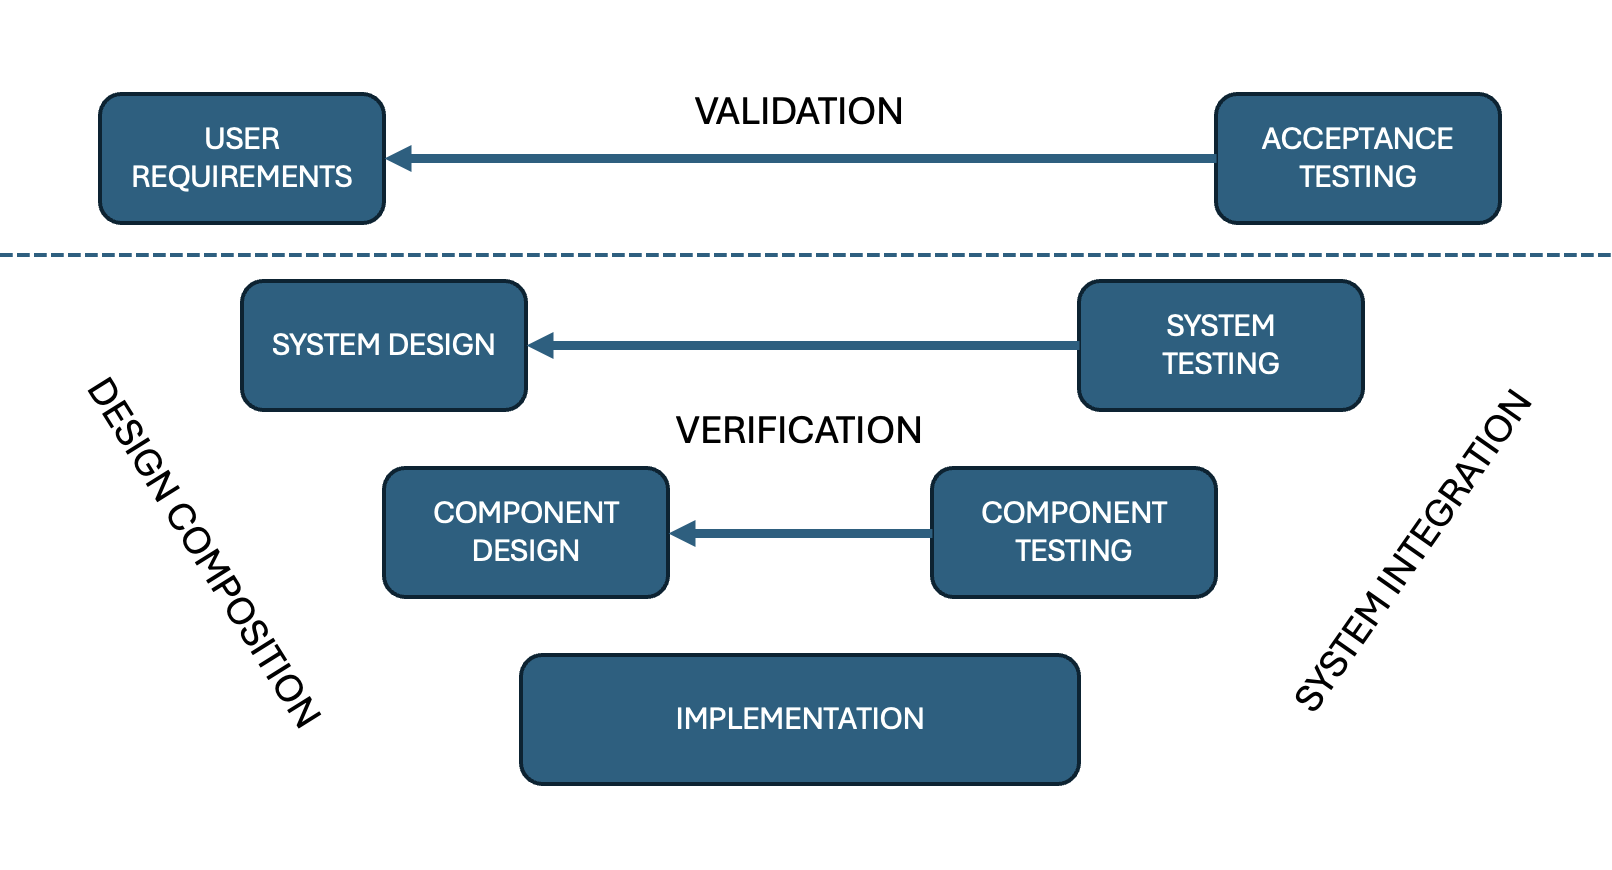
\includegraphics{v_model_methodology.png}
  \caption{Methodological framework based on the V-model from \glsentryshort{incose} with the different stages of the project development process\autocite{ruddle2020vmodel}}\label{fig:v_model_methodology}
\end{figure}

The V-model provides a structured approach to project development, ensuring that all aspects of the project are considered and addressed. By following this methodological framework, this research aims to develop a comprehensive and effective solution for the design and implementation of a fully distributed parking management system tailored for the next generation of smart cities.

% Local Variables:
% jinx-local-words: "incose"
% End:
